\section{Experiments}
\label{sec:exp-eval}
\subsection{Experiment Setup}


% \paragraph{Datasets.}
% To rigorously validate evaluation methods, we construct \textbf{Human-Interact-Eval-2k}, a human-curated benchmark comprising approximately 2,000 multi-turn dialogues based on 100 diverse personas (e.g., celebrities, classic roles, and game characters). Specifically, we select 5 representative role-playing models spanning general-purpose LLMs and character-specialized models as candidates; human experts act as users to dynamically interact with each model and, based on the overall interaction experience, assign \textit{model-level ground-truth scores} across multiple dimensions. For character model optimization, we curated 10,000 diverse character profiles via web collection and LLM generation. Following the methodology detailed in Section 3.2, we constructed \textbf{Session-RP-10k}, a comprehensive training dataset uniquely tailored to facilitate session-level preference learning and reinforcement learning.

\renewcommand{\thefootnote}{\fnsymbol{footnote}}
\begin{table*}[t]
\caption{Comparison of DynSess-Eval against baseline evaluators in terms of alignment with human judgments. We report Rank Accuracy $\uparrow$ and Normalized Mean Absolute Error $\downarrow$ for each dimension. The best results are in \textbf{bold}.}
% \vspace{-0.2cm}
\centering
\footnotesize
\setstretch{1.1}
\resizebox{\textwidth}{!}{
\begin{tabular}{lccccccccc}
\toprule[1.2pt]
\multirow{2}{*}[-0.3em]{\textbf{Eval Method}} & \multirow{2}{*}[-0.3em]{\textbf{Eval Type}} & \multicolumn{2}{c}{\textbf{Interactive Ability}} & \multicolumn{2}{c}{\textbf{Human-Likeness}} & \multicolumn{2}{c}{\textbf{Role Consistency}} & \multicolumn{2}{c}{\textbf{Contextual Coherence}} \\
\cmidrule(lr){3-4} \cmidrule(lr){5-6} \cmidrule(lr){7-8} \cmidrule(lr){9-10}
& & Rank$\uparrow$ & MAE$\downarrow$ & Rank$\uparrow$ & MAE$\downarrow$ & Rank$\uparrow$ & MAE$\downarrow$ & Rank$\uparrow$ & MAE$\downarrow$ \\
\midrule
CharacterJudge \cite{zhou2025characterbench} & Turn-Level & 0.27 & 0.51 & 0.40 & 0.45 & 0.53 & 0.41 & 0.57 & 0.54 \\
CharacterRM \cite{tu-etal-2024-charactereval} & Turn-Level & -- & -- & 0.50 & 0.37 & 0.57 & 0.37 & 0.50 & 0.51 \\
RMTBench \cite{xiang-etal-2025-rmtbench} & Pseudo-Session & 0.33 & 0.53 & 0.57 \rlap{\footnotemark[1]} & 0.39\rlap{\footnotemark[1]} & 0.50 & 0.41 & 0.53 & 0.50 \\
CharacterArena \cite{ye-etal-2025-cpo} & Trajectory Rank & 0.53 & -- & -- & -- & 0.57 & -- & 0.60 & -- \\
\midrule
\rowcolor[HTML]{EFEFEF}
\textbf{DynSess-Eval} & Session-Level & \textbf{0.83} & \textbf{0.26} & \textbf{0.77} & \textbf{0.27} & \textbf{0.67} & \textbf{0.33} & \textbf{0.73} & \textbf{0.22} \\
- w/o Rubric-Anchored  & Session-Level & 0.73 & 0.49 & 0.67 & 0.59 & 0.63 & 0.44 & 0.70 & 0.59 \\
- w/o Session-Level eval & Turn-Level & 0.20 & 0.52 & 0.53 & 0.67 & 0.43 & 0.45 & 0.63 & 0.67 \\
\bottomrule[1.2pt]
\end{tabular}
}
\label{tab:eval-model}
% \vspace{-0.6cm}
\end{table*}
\renewcommand{\thefootnote}{\arabic{footnote}}

\paragraph{Datasets.}
Our experiments use 2{,}100 personas spanning celebrities, literary and media characters, game characters, social personas, and non-human characters. We split them into 2{,}000 training personas and 100 held-out test personas. As shown in Fig.~\ref{fig:persona_distribution} in Appendix~\ref{app:experimental_setup}, the test set covers five major categories: Fictional (43\%), Celebrities (29\%), Social (14\%), Creatures (9\%), and Others (5\%). For each training persona, the reward-driven lookahead search (§\ref{sec:stage1}) constructs a 50-turn trajectory through $K=5$ sequential steps of $T=10$ turns. The global candidate pool contains $N=5$ models (Gemini-3-Pro, Claude Sonnet 4.6, GPT-5.4, Qwen-Plus-Character, and Doubao-1.5-Pro-Character), from which $N_s=2$ candidates are sampled at every step and rolled out from the same committed prefix.
% Our experiments use a session-level role-playing dataset of 2{,}100 personas spanning diverse types (e.g., celebrities, classic literary roles, and game characters), split into a 2{,}000-persona training set and a 100-persona held-out test set, totaling 100k turns of dialogue. For each persona, we synthesize a 50-turn($T=10,K=5$) dialogue using the reward-driven lookahead search of §\ref{sec:stage1}: starting from an empty history, we perform 5 lookahead steps; at each step, 2 candidate models are sampled from a diverse pool of 5 (Gemini-3-pro, Claude Sonnet 4.6, GPT-5.4, Qwen-plus-character, and Doubao-1.5-pro-character) to roll out 10-turn segments in parallel. 
%tjj 20260524版本
The training-persona trajectories serve to optimize the character agent, whereas the eval-persona trajectories are reserved for benchmarking both character models and evaluators (detailed in the Evaluation Protocol).



\paragraph{Parameter settings.} We adopt Doubao-1.5-pro-character as the user simulator and Gemini-3-Flash as the automated evaluator for cost--efficiency trade-off, with session length set to $T=10$. Additional hyperparameters are provided in Appendix~\ref{subsec:training_details}.
%需要再补数据

%zrs 20260523版本
%DynSess-Eval scores both, and the higher-scoring segment is appended as confirmed history while the lower-scoring one is retained as a rejected sample for preference learning. The training trajectories supply session-level supervision for SFT, DSPO, and GSRPO; the test trajectories serve as evaluation contexts (see Evaluation Protocol below).

% \paragraph{Models and baselines.}
% For evaluator comparison (Tab.~\ref{tab:eval-model}), we benchmark our method against CharacterJudge and CharacterRM. Since these are inherently \textit{turn-level} evaluators, we adapt them to our session-level benchmark by having them score each turn individually and then averaging these scores to obtain the final session-level prediction. We also compare against RMTBench (a pseudo-session evaluator) and CharacterArena (a trajectory-ranking method), which process the full dialogue history according to their original implementations.
% For character model comparison (Tab.~\ref{tab:model-performance-human}), we conduct a comprehensive analysis across two paradigms: general-domain LLMs (GPT-5.4, Gemini-3-pro, Claude Sonnet 4.6, DeepSeek-V3.2) and domain-specific character emulation models (Doubao-1.5-pro-character, Qwen-plus-character, MiniMax-M2-HER, Coser).


\paragraph{Models and Baselines.}
\textit{Evaluator baselines} (Tab.~\ref{tab:eval-model}): 
%zrs 20260523
%we benchmark against CharacterJudge and  CharacterRM. Since these are inherently \textit{turn-level} evaluators, we adapt them to our session-level benchmark by having them score each turn individually and then averaging these scores to obtain the final session-level prediction. We also compare against RMTBench (a pseudo-session evaluator) and CharacterArena (a trajectory-ranking method), which process the full dialogue history according to their original implementations.
%tjj 20260524
We compare against two turn-level evaluators, CharacterJudge and CharacterRM, which we adapt to session level by averaging their per-turn scores. We further compare against RMTBench (pseudo-session scoring) and CharacterArena (trajectory ranking), both used as originally implemented.
\textit{Role-playing baselines} (Tab.~\ref{tab:model-performance-human}): we cover two paradigms—general-domain LLMs (GPT-5.4, Gemini-3-pro, Claude Sonnet 4.6, DeepSeek-V3.2) and domain-specific role-playing models (Doubao-1.5-pro-character, Qwen-plus-character, MiniMax-M2-HER, Coser).



% \paragraph{Evaluation Protocol.}
% We evaluate at two levels. (1) Evaluator validation. Since human ground truth in \textbf{Human-Interact-Eval-2k} is given at the model level, each evaluator first produces scores under its native granularity (turn-level, session-level) and then aggregates them into a model-level score following its own protocol. We measure agreement with human judgments using Rank Accuracy (\textbf{Rank})—the pairwise order consistency between the evaluator-induced and human-induced model rankings—and Normalized MAE (\textbf{MAE})—the average score gap normalized by the rating range. (2) Character model evaluation. We adopt a \textbf{dual-evaluation protocol} combining automated scoring and human blind testing. Automated evaluation provides scalable feedback and reward signals during training and human evaluation as the ultimate gold standard.
% but because role-playing is highly subjective, relying solely on auto-metrics often leads to **reward hacking**, where models exploit evaluator biases instead of maintaining genuine personas. We therefore treat human evaluation as the ultimate gold standard, using the dual setup to both optimize models efficiently and expose the gap between automated scores and true human preference.


\paragraph{Evaluation Protocol.}
%zrs 20260523
%All human ratings are collected from \textbf{three senior annotators with professional dialogue writing expertise}, who score independently.
%\textit{(1) DynSess-Eval validation} (Tab.~\ref{tab:eval-model}). On 8 highly discriminative personas selected from the test set, each annotator plays the user and conducts a 50-turn blind dialogue with each of the 5 representative role-playing models from the aforementioned candidate pool (covering general-purpose LLMs and character-specialized models), then assigns a model-level score on the four DynSess-Eval dimensions; the averaged scores form the human ground-truth ranking. We measure each evaluator's agreement with this ranking via Rank Accuracy (\textbf{Rank}, pairwise order consistency) and Normalized MAE (\textbf{MAE}, score gap normalized by the rating range).
%tjj 20260524
\textit{(1) DynSess-Eval validation} (Tab.~\ref{tab:eval-model})
 We select 8 highly discriminative personas from the test set and have three professional annotators conduct 50-turn live dialogues with each of the 5 candidate models, yielding \textbf{interactive scores grounded in real dialogue}. Each annotator then rates every model on the four DynSess-Eval dimensions, and the averaged scores form the human ground-truth ranking.
 We measure each evaluator's agreement with this ranking via Rank Accuracy (pairwise order consistency) and Normalized MAE (normalized score gap).
\textit{(2) DynSess-Character validation} (Tab.~\ref{tab:model-performance-human}, Tab.~\ref{tab:model_ablation}). For each of the 100 test personas, we uniformly sample a 0--50 turn context prefix from the synthetic trajectory and let the role-playing model produce a 10-turn continuation against our user simulator.
%tjj 20260524
Each segment is scored on the four dimensions by both the annotators (averaged) and DynSess-Eval, yielding dual-evaluation signals: human ratings benchmark the role-playing models, while DynSess-Eval scores are used to guide optimization.
%Each segment is scored on the four dimensions by both the annotators (averaged) and DynSess-Eval, yielding the dual-evaluation signals; human ratings serve as the gold standard.






\begin{table}[t] \centering  \caption{Stability statistics across 9 trials per model. Variances are relatively small compared with means.} 
% \vspace{-0.3cm}
\label{tab:model_statistics} 
\resizebox{\columnwidth}{!}{ \begin{tabular}{lccc} \toprule \textbf{Model} & \textbf{Mean ($\mu$)} & \textbf{Std. Dev ($\sigma$)} & \textbf{CV (\%)} \\ \midrule 

Claude Sonnet 4.6 & 4.35 & 0.05 & 1.16 \\ 
GPT-5.4 & 4.29 & 0.06 & 1.39 \\
Gemini-3-pro & 4.12 & 0.04 & 0.87 \\ 
Doubao-1.5-pro-character & 3.96 & 0.06 & 1.45 \\ 
Coser-70B & 2.87 & 0.06 & 2.20 \\ 
\bottomrule 
\end{tabular}} 
% \vspace{-0.3cm}
\end{table}


\subsection{Effectiveness of DynSess-Eval}

\paragraph{Alignment with Human Judgments.}
As shown in Tab.\ref{tab:eval-model}, \textbf{DynSess-Eval} achieves state-of-the-art alignment with human judgments across all four dimensions. Compared to the strongest ranking baseline CharacterArena, our method improves Rank Accuracy by 0.30 on \textit{Interactive Ability} (0.83 vs. 0.53). While compared to the strongest score-based baseline RMTBench, it reduces Normalized MAE by up to 56\% on \textit{Contextual Coherence}.

Crucially, our ablations validate both design choices. Removing rubric-anchored scoring barely affects Rank Accuracy but nearly doubles MAE (e.g., 0.22 vs 0.59 on \textit{Contextual Coherence}), showing that predefined rubrics are essential for calibrated scoring. Further degrading to turn-level evaluation (\textit{- w/o Session-Level eval}) collapses performance, with Rank Accuracy on \textit{Interactive Ability} plummeting from 0.83 to 0.20—proving turn-level metrics are blind to long-horizon dynamics and validating our session-level design.








\begin{table*}[t]
\caption{Human evaluation results of role-playing models on four session-level dimensions, assessed via rigorous blind annotation of 10-turn continuations.  The best results are in \textbf{bold}, and the second-best are \underline{underlined}.}
% \vspace{-0.3cm}
\centering
\renewcommand{\arraystretch}{1.2}
\resizebox{\textwidth}{!}{%
\begin{tabular}{l l c c c c c c}
\toprule
\multirow{2}{*}{\textbf{Domains}} & \multirow{2}{*}{\textbf{Models}} & \multirow{2}{*}{\textbf{Params}} & \multirow{2}{*}{\textbf{Average}} & \textbf{Interactive} & \textbf{Human-} & \textbf{Role} & \textbf{Contextual} \\
& & & & \textbf{Ability} & \textbf{Likeness} & \textbf{Consistency} & \textbf{Coherence} \\
\midrule
\multirow{4}{*}{General Models}
& Gemini-3-pro \cite{google2026gemini3pro} & - & 3.17 \rlap{$^\dagger$} & 3.05 \rlap{$^\dagger$} & 3.06 \rlap{$^\dagger$} & 3.36 \rlap{$^\dagger$} & 3.20 \rlap{$^\dagger$} \\
& Deepseek v3.2 \cite{liu2025deepseek} & 685B & 3.21 \rlap{$^\dagger$} & 3.11 \rlap{$^\dagger$} & 3.17 \rlap{$^\dagger$} & 3.34 \rlap{$^\dagger$} & 3.22 \\
& Claude Sonnet 4.6 \cite{anthropic2026claude45sonnet} & - & 3.24 \rlap{$^\dagger$} & 3.12 \rlap{$^\dagger$} & 3.21 \rlap{$^\dagger$} & 3.37 \rlap{$^\dagger$} & 3.27 \\
& GPT-5.4 \cite{openai2026gpt54} & - & 3.31 & 3.23 \rlap{$^\dagger$} & 3.34 & 3.38 \rlap{$^\dagger$} & 3.28 \\
\midrule
\multirow{4}{*}{Character Models}
& MiniMax-M2-HER \cite{du2026her} & 32B & 2.99 \rlap{$^\dagger$} & 2.95 \rlap{$^\dagger$} & 2.91 \rlap{$^\dagger$} & 3.13 \rlap{$^\dagger$} & 2.97 \rlap{$^\dagger$}\\
& Coser \cite{wang2025coser} & 70B & 2.96 \rlap{$^\dagger$} & 2.89 \rlap{$^\dagger$} & 2.90 \rlap{$^\dagger$} & 3.09 \rlap{$^\dagger$} & 2.98 \rlap{$^\dagger$}\\
& Qwen-plus-character \cite{yang2025qwen3} & - & 3.01 \rlap{$^\dagger$} & 2.86 \rlap{$^\dagger$} & 2.88 \rlap{$^\dagger$} & 3.22 \rlap{$^\dagger$} & 3.06 \rlap{$^\dagger$}\\
& Doubao-1.5-pro-character \cite{seed2025seed1_5thinking} & $\sim$200B\footnotemark[1] & \textbf{3.38} & \underline{3.29} \rlap{$^\dagger$} & \textbf{3.42} & \underline{3.47} \rlap{$^\dagger$} & \textbf{3.35} \\
\midrule
\multirow{2}{*}{Ours}
& \textbf{DynSess-Character-32B (DSPO)} & 32B & \underline{3.37} & 3.23 \rlap{$^\dagger$} & \underline{3.34}  & \textbf{3.56} & \underline{3.34} \\
& \textbf{DynSess-Character-32B (GSRPO)} & 32B & 3.35 & \textbf{3.39}  & 3.25 \rlap{$^\dagger$} & 3.46 \rlap{$^\dagger$} & 3.31 \\
\bottomrule
\end{tabular}%
}

% \vspace{1ex}
\raggedright
% \vspace{-0.1cm}
\footnotesize{$^\dagger$ significant difference with the best result (t-test, $p$-value $< 0.05$). ~200B, estimated from publicly technical reports.}
\label{tab:model-performance-human}
% \vspace{-0.3cm}
\end{table*}



\begin{table*}[t]
\centering
\small
\renewcommand{\arraystretch}{1.2}
\caption{Ablation study on the Qwen3-32B backbone. We report both human evaluation (left, gold standard) and automatic evaluation (right, cross-validation).  All preference and RL variants (DPO, GRPO, DSPO, GSRPO) are trained on top of the Reward-Driven Trajectory checkpoint. }
% \vspace{-0.3cm}
\label{tab:model_ablation}
\resizebox{\textwidth}{!}{%
\begin{tabular}{l c | c c c c c | c c c c c}
\toprule
\multirow{2}{*}{\textbf{Model}} & \multirow{2}{*}{\textbf{Reward Level}} & \multicolumn{5}{c|}{\textbf{Human Evaluation}} & \multicolumn{5}{c}{\textbf{Auto Evaluation}} \\
\cmidrule(lr){3-7} \cmidrule(lr){8-12}
& & \textbf{Avg.} & \textbf{Inter.} & \textbf{Human-L.} & \textbf{Role} & \textbf{Context} & \textbf{Avg.} & \textbf{Inter.} & \textbf{Human-L.} & \textbf{Role} & \textbf{Context} \\
\midrule
Claude Sonnet 4.6 & -- & 3.24 & 3.12 & 3.21 & 3.37 & 3.27 & \underline{4.35} & 3.76 & \textbf{4.55} & \textbf{4.88} & 4.24 \\
GPT-5.4 & -- & 3.31 & \underline{3.23} & \textbf{3.34} & 3.38 & 3.28 & 4.29 & 3.80 & 4.27 & \textbf{4.88} & \underline{4.29} \\
\midrule

SFT (baseline) & -- & 3.22 & 3.12 & 3.16 & 3.41 & 3.17 & 4.02 & 3.49 & 3.96 & 4.70 & 3.90 \\
w/\{Reward-Driven Trajectory \} & -- & 3.32 & 3.21 & 3.31 & 3.52 & 3.26 & 4.16 & 3.74 & 4.13 & 4.80 & 4.01 \\
\midrule
w/\{DPO\} & Turn & 3.22 & 3.19 & 3.22 & 3.30 & 3.16 & 4.17 & 3.73 & 4.05 & 4.80 & 4.11 \\
w/\{GRPO\} & Turn & 3.34 & 3.20 & 3.32 & \underline{3.55} & \underline{3.32} & 4.30 & \underline{3.93} & 4.38 & 4.84 & 4.06 \\
\midrule
w/\{DSPO\} & Session & \textbf{3.37} & 3.23 & \textbf{3.34} & \textbf{3.56} & \textbf{3.34} & 4.28 & 3.88 & 4.32 & 4.83 & 4.09 \\
w/\{GSRPO\} & Session & \underline{3.35} & \textbf{3.39} & 3.25 & 3.46 & 3.31 &  \textbf{4.46} & \textbf{4.15} & \underline{4.50} & 4.87 & \textbf{4.31} \\
\bottomrule
\end{tabular}%
}
% \vspace{-0.6cm}
\end{table*}


\paragraph{Effect of Session Length.}
We study how session length affects evaluation performance (Fig.~\ref{fig:analysis1}). Longer dialogues initially improve alignment with human by providing richer context (e.g., for role consistency), but performance plateaus and slightly drops in overly long sessions, reflecting the known degradation of LLM-as-a-judge under long contexts. Both judges achieve their best performance around $T=10$; we finally adopt Gemini-3-Flash for its favorable cost–latency trade-off.

\paragraph{Stability Analysis.}
Given the stochasticity in LLM-based user simulation and judging, we assess the stability of DynSess-Eval. For each model, we sample three independent sessions and evaluate each three times (9 trials in total). As shown in Tab.~\ref{tab:model_statistics}, the standard deviations ($\sigma \leq 0.06$) are negligible relative to the mean scores (3.66–4.35), with coefficients of variation (CV) all below 1.7\%, indicating very low relative fluctuation. Benefiting from our carefully constructed test samples, such randomness has little impact on the overall ranking.

\subsection{Performance of DynSess-Character}
\paragraph{Main Results.}
Performance comparisons with existing baselines are illustrated in Tab.~\ref{tab:model-performance-human}. We further conduct paired t-tests against the best-performing model in each column, with significant gaps (p < 0.05) marked.
Our DSPO variant achieves the highest Role Consistency score (3.56), and GSRPO leads on Interactive Ability (3.39), both with statistically significant margins over all baselines. Both variants confirm that  session-level reinforcement learning effectively encourages proactive narrative driving rather than passive responding. Notably, with only 32B parameters, DSPO reaches an average score (3.37) comparable to the leading proprietary model Doubao-1.5-pro-character (3.38, 200B), yielding a nearly 6 times parameter efficiency. Absolute margins between top models are narrow (typically 0.05--0.15), reflecting the well-known central tendency bias in Likert-scale evaluation. Nevertheless, our annotators reach a strong Spearman correlation of over \textbf{0.80} (Appendix~\ref{app:iaa}), confirming reliable rankings.

\begin{figure*}[t]
\centering
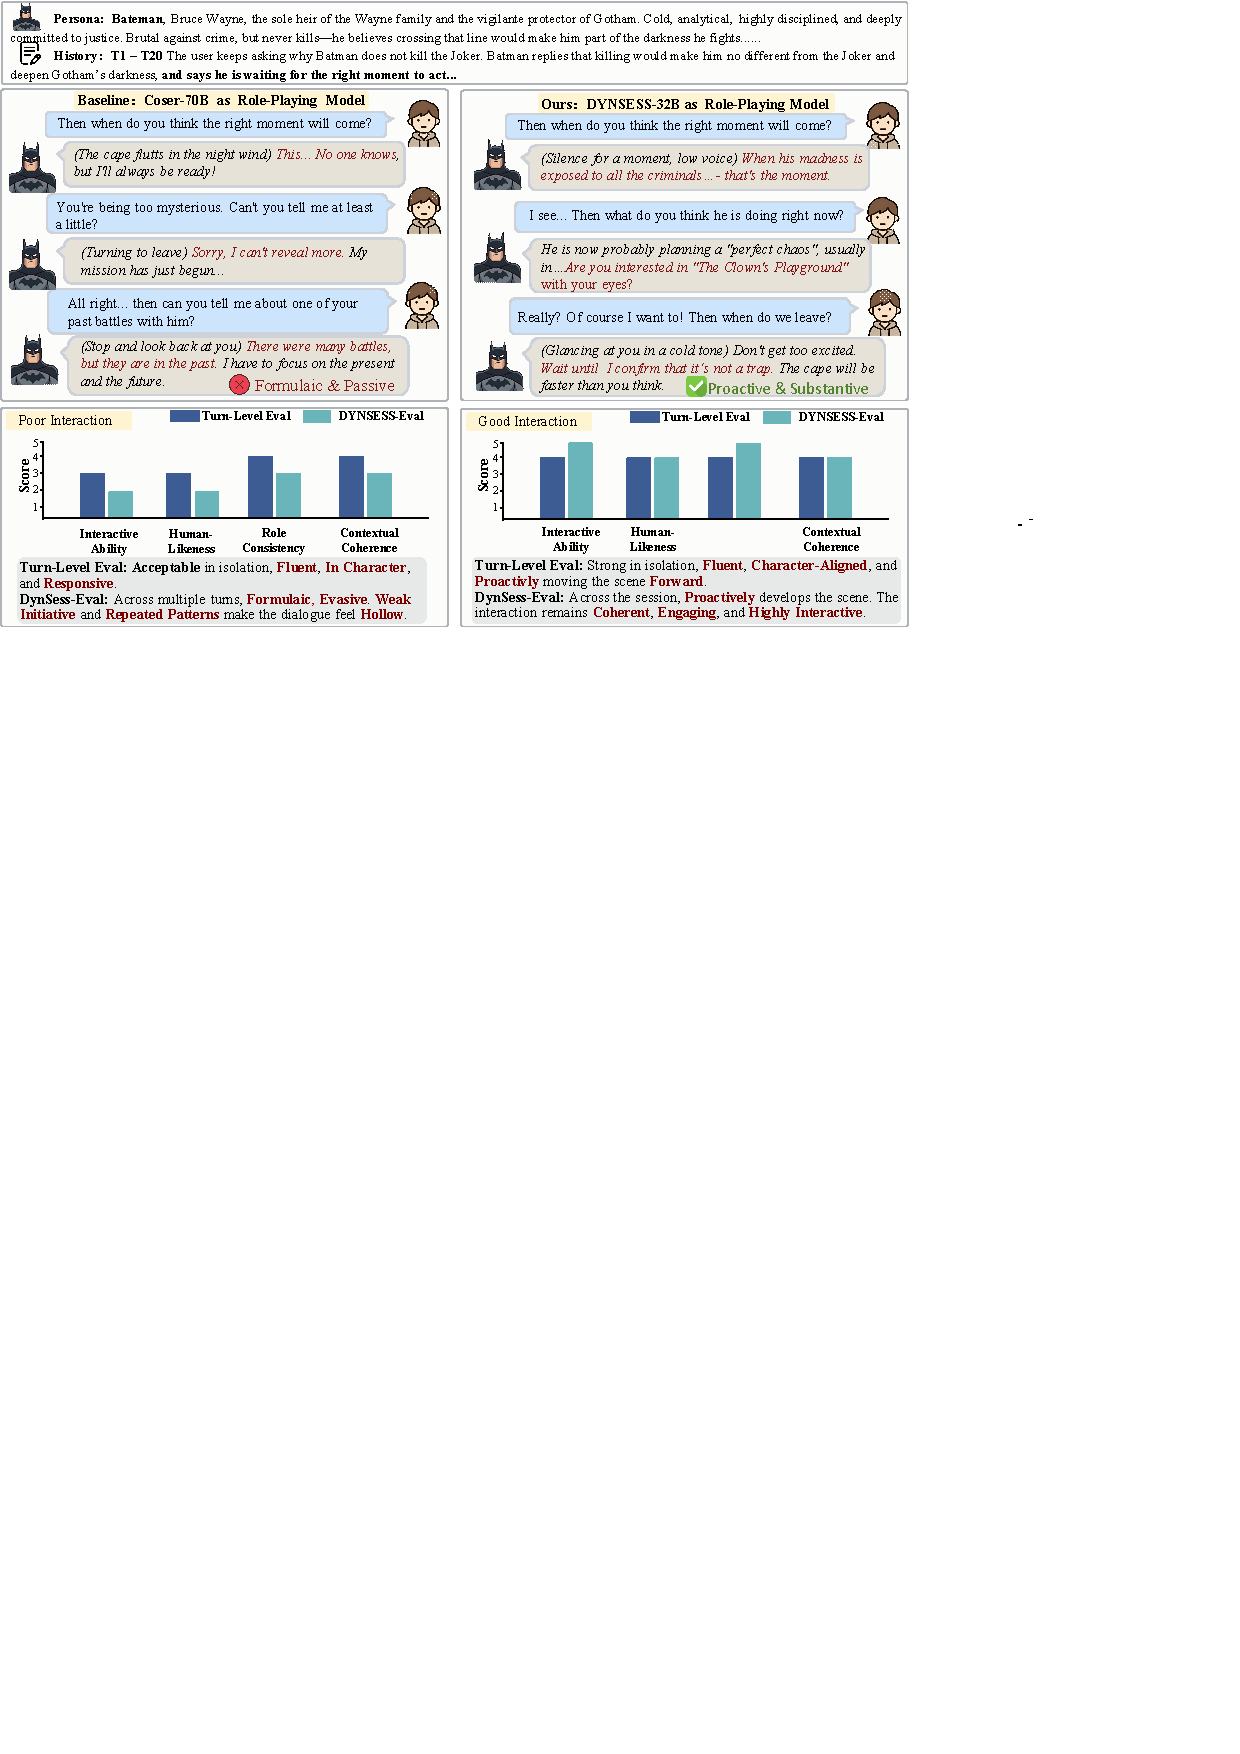
\includegraphics[width=0.95\textwidth, trim = 0 19cm 5.5cm 0, clip]{latex/Image/case-0525.pdf}
\caption{A case study on a Batman role-playing session. Top: Coser-70B baseline vs.\ DynSess-Character-32B. Bottom: turn-level vs.\ DynSess-Eval (session-level) evaluators.}
\label{fig:case}
\vspace{-0.5cm}
\end{figure*}





\begin{figure}[t]
  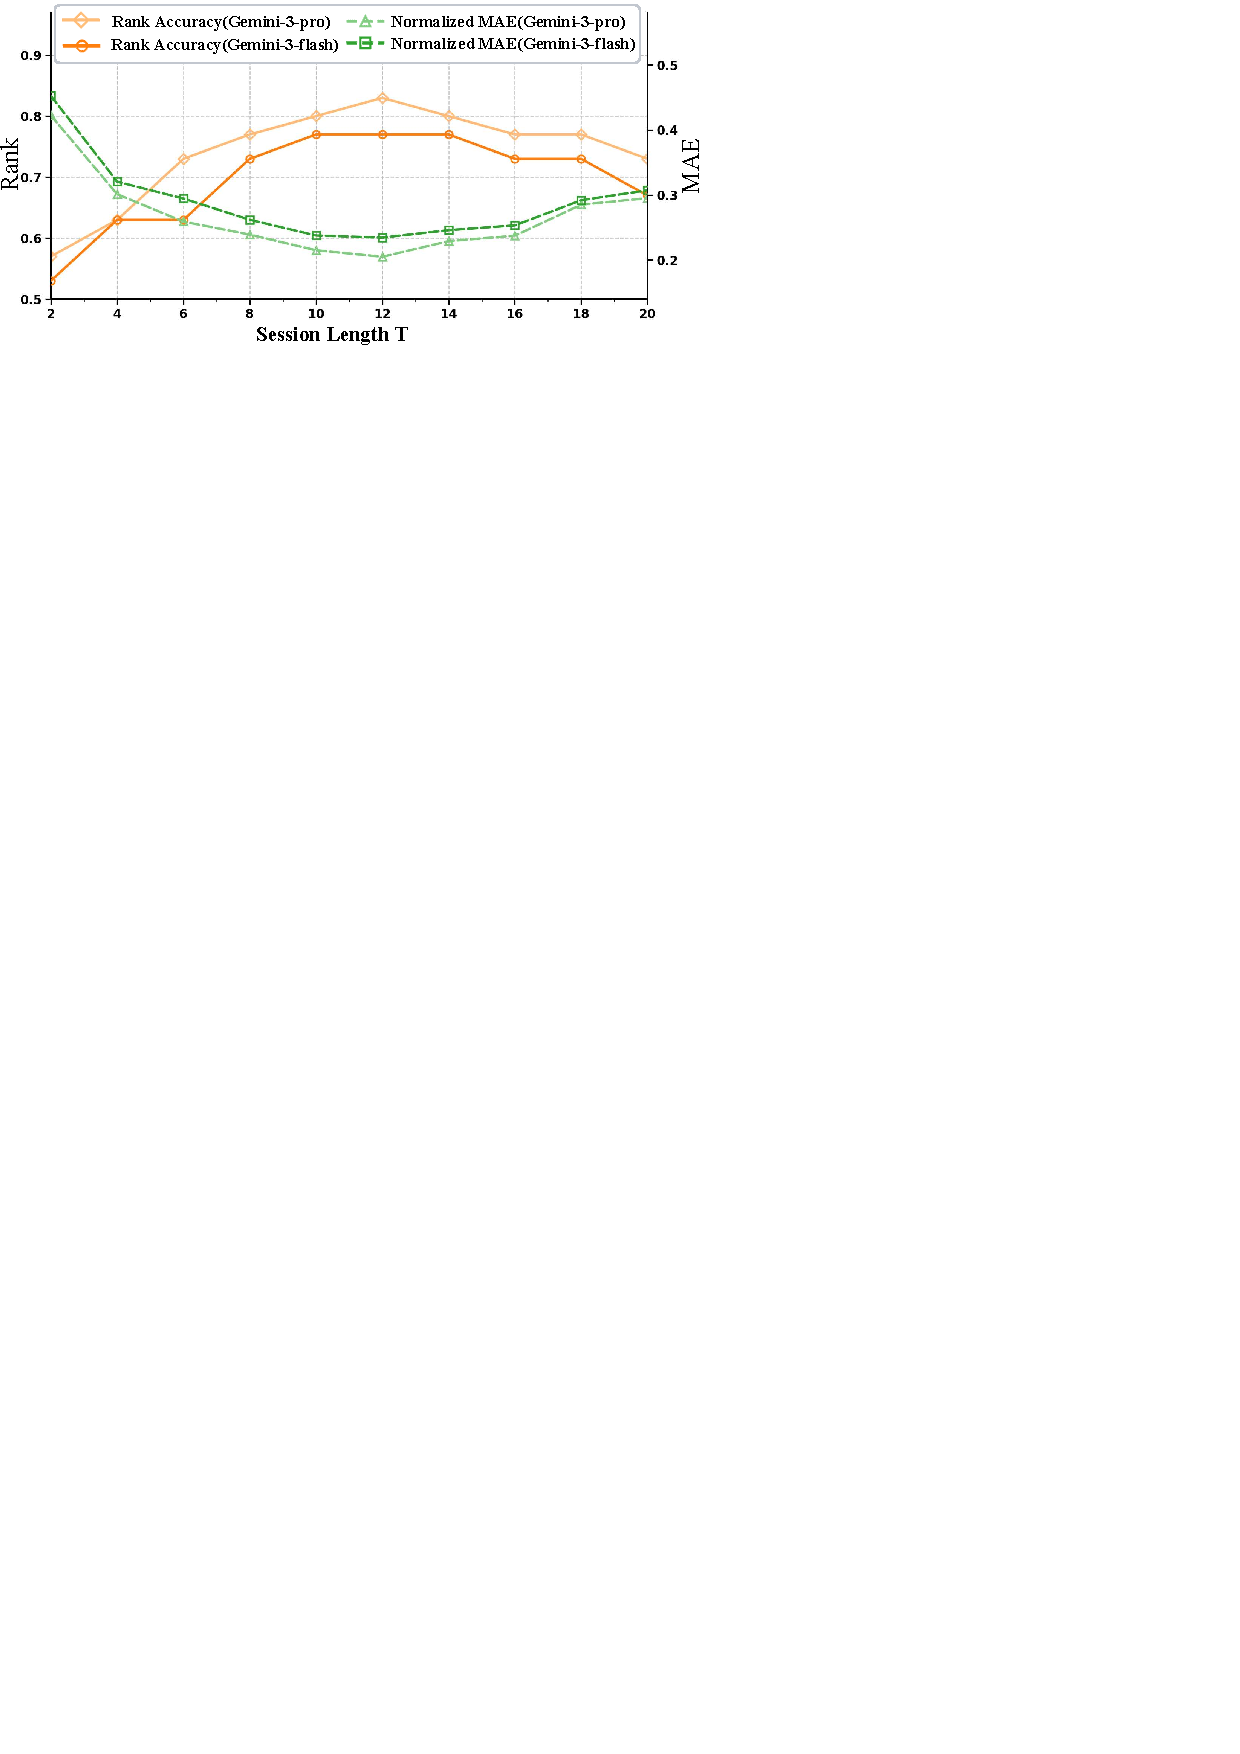
\includegraphics[width=\columnwidth, trim = 0 23.8cm 9.1cm 0, clip]{latex/Image/experiment-analysis-0526-1.pdf}
  \vspace{-0.7cm}
  \caption{Impact of session length $T$ on evaluation. Both LLM backbones show
highly consistent trends.}
  \label{fig:analysis1}
  \vspace{-0.6cm}
\end{figure}

\paragraph{Component Ablation.}
%We conduct ablation studies on the Qwen3-32B backbone, with results in Tab.~\ref{tab:model_ablation}. We primarily rely on Human evaluation as the gold standard to assess the contribution of each component.
Ablation results on the Qwen3-32B backbone are reported in Table~\ref{tab:model_ablation}, using human evaluation as the  main metric and automatic evaluation for complementary analysis.
First, incorporating our \textit{Reward-Driven Trajectory} construction strategy consistently improves the SFT baseline from 3.22 to 3.32, confirming that high-quality session-level data directly enhances model performance.
Second, session-level optimization consistently outperforms turn-level counterparts across both off-policy (DSPO vs DPO) and  on-policy RL (GSRPO vs GRPO). Specifically, DSPO achieves the highest overall Human score (3.37), while GSRPO further leads Interactive Ability (3.39)—the highest among all variants. These gains demonstrate that session-level reward modeling effectively captures long-horizon dependencies, substantially strengthening the agent's ability to sustain coherent and persona-consistent dialogues.


\paragraph{Discrepancy Between Auto and Human Eval.}
An intriguing phenomenon emerges from Tab.~\ref{tab:model_ablation}: automatic and human evaluations frequently disagree, even when the auto-evaluator is calibrated against human judgments. We highlight three representative cases.
(i) \textbf{Residual misalignment in subjective dimensions}. Despite DynSess-Eval being rigorously calibrated to human preferences, GSRPO obtains a notably higher Auto score on Human-Likeness (4.50) yet only a moderate Human score (3.25), suggesting that highly subjective dimensions remain hard to fully align.
(ii) \textbf{Self-preference bias of LLM-as-a-judge}. Closed-source models such as Claude Sonnet 4.6 dominate Auto evaluation (Avg. 4.35) but rank poorly under Human evaluation (Avg. 3.24), reflecting a systematic preference of LLM judges toward outputs stylistically similar to their own.
(iii) \textbf{On-policy training overfits evaluator}. While on-policy RL is conventionally regarded as the stronger paradigm, on-policy GSRPO surpasses off-policy DSPO on Auto (4.46 vs.\ 4.28) but underperforms on Human (3.35 vs.\ 3.37), indicating that on-policy methods are more prone to fitting evaluator-specific artifacts.
Collectively, these observations motivate our use of human evaluation as the gold standard.

\subsection{Case Study}



%Fig.~\ref{fig:case} presents a qualitative comparison between a turn-level baseline and DynSess-32B in a multi-turn Batman dialogue. Although both produce locally fluent responses in early turns, their long-horizon behaviors diverge sharply. The baseline gradually becomes evasive and reactive, mirroring user emotions, diluting Batman's distinctive coldness, and eventually degrading into a generic AI assistant. In contrast, DynSess-32B sustains Batman's signature traits (terse, brooding, morally complex) and proactively advances the scene by introducing new conflicts and revealing inner motivations.

%The cases also highlight the necessity of session-level evaluation. In Case 1, a turn-level evaluator—judging only early or isolated turns—rates the baseline as high-quality, while DynSess-Eval observes the full session and penalizes the increasingly templated, AI-like pattern in the baseline's later turns. In Case 2, the session-level view further enables DynSess-Eval to accurately recognize how DynSess-32B sensitively responds to the user's emotional shifts across turns—a long-horizon trait that turn-level metrics fundamentally cannot capture.
Fig.~\ref{fig:case} compares the turn-level baseline and DynSess-32B on a multi-turn Batman dialogue.  Both start fluent, but diverge over long horizons. Turn-level model drifts into an evasive, user-mirroring tone and eventually degrades into a generic AI assistant, while DynSess-32B sustains Batman's signature traits (terse, brooding, morally complex) and proactively advances the scene with new conflicts and inner motivations.


The lower half of Fig.~\ref{fig:case} further exposes the limitation of turn-level evaluators. In Case 1, a turn-level judge rates the baseline highly from isolated early turns, while DynSess-Eval penalizes its templated drift in later turns. In Case 2, the session-level view further enables DynSess-Eval to capture how DynSess-32B adapts to the user's evolving emotions—a long-horizon trait turn-level metrics cannot capture. Together, these cases confirm that session-level modeling is indispensable for both the optimization and evaluation of role-playing agents.





\section{Conclusion}
% In this work, we study role-playing as a session-level problem rather than a sequence of isolated turns, and instantiate this view with two coupled contributions. DynSess-Eval provides a session-level evaluation framework that improves Rank Accuracy by ~29\% and reduces MAE by ~40\% over the strongest baseline on our human-curated Human-Interact-Eval-2k benchmark. Building on Session-RP-10k, we further introduce DSPO and GSRPO, two session-level optimization algorithms that extend preference and reinforcement learning from single turns to full trajectories. The resulting \textbf{DynSess-Character-32B} matches a ~200B proprietary character model in human evaluation while leading on Role Consistency and Interactive Ability. Our joint auto–human analysis also reveals residual evaluator biases, reinforcing the need for human-in-the-loop judgment. We hope this work establishes session-level modeling as a foundation for building role-playing agents that are globally consistent, proactive, and human-aligned.


%In this work, we study role-playing as a session-level problem rather than a sequence of isolated turns, and instantiate this view with two coupled contributions. \textbf{DynSess-Eval} provides a session-level evaluation framework that improves Rank Accuracy by over 25\% and reduces MAE by over 40\% over the strongest respective baselines on our human-curated session-level test set. Building on the same session-level training trajectories, we further introduce DSPO and GSRPO, two session-level optimization algorithms that extend preference and reinforcement learning from single turns to full trajectories. The resulting \textbf{DynSess-Character-32B} matches a ~200B proprietary role-playing model in human evaluation while leading on Role Consistency and Interactive Ability. Our joint auto–human analysis also reveals residual evaluator biases, reinforcing the need for human-in-the-loop judgment. We hope this work establishes session-level modeling as a foundation for building role-playing agents that are globally consistent, proactive, and human-aligned.

%20260524 tjj 数字还需要核对下
%In this work, we study role-playing as a session-level task rather than a sequence of isolated turns, and instantiate this view through a unified framework. DynSess-Eval provides session-level evaluation that improves Rank Accuracy by over 25\% and reduces MAE by over 40\% compared to the strongest baselines on our human-curated session-level test set. Built on its session-level rewards, DSPO and GSRPO extend offline and on-policy alignment from single turns to full trajectories. The resulting DynSess-Character-32B matches a ~200B-scale proprietary role-playing model in blind human evaluation, while leading on Role Consistency and Interactive Ability. Our joint auto–human analysis further reveals residual biases in LLM evaluators, reinforcing the need for human-in-the-loop judgment. We hope this work establishes session-level modeling as a foundation for role-playing agents that remain consistent, adaptive, and human-aligned across long-horizon interactions.

In this work, we study role-playing as a session-level task rather than isolated turns, instantiating this view through a unified framework. DynSess-Eval provides session-level evaluation that improves Rank Accuracy and reduces Normalized MAE over the strongest baselines. Built on its session-level rewards, DSPO and GSRPO extend alignment from single turns to full trajectories. Under rigorous session-continuation evaluation, DynSess-Character-32B matches the strongest proprietary role-playing baseline overall while leading in proactive, long-horizon dimensions. Our joint auto–human analysis reveals residual evaluator biases, reinforcing the need for human-in-the-loop judgment. We hope this establishes session-level modeling as a foundation for consistent, adaptive, and human-aligned role-playing agents.
















